\documentclass[aos,noinfoline]{imsart} % annals of applied statistics 
\setattribute{journal}{name}{} 

\RequirePackage[OT1]{fontenc}
\RequirePackage{amsthm,amsmath,amssymb}
\RequirePackage[square,authoryear,sort]{natbib}
\RequirePackage[authoryear]{natbib}
\RequirePackage[colorlinks,citecolor=blue,urlcolor=blue]{hyperref}

% settings
%\pubyear{2014}
%\volume{0}
%\issue{0}
%\firstpage{1}
%\lastpage{8}
%\arxiv{arXiv:0000.0000}

\usepackage{../macros}
\usepackage{fullpage}
\usepackage[mathcal, mathscr]{eucal}
\usepackage{verbatim}
\usepackage{colortbl}
\usepackage[size=small]{caption}
\usepackage{subcaption}
\usepackage{graphicx}
\graphicspath{{../figures/}}
\DeclareGraphicsExtensions{.pdf,.png,.jpg,.eps}
\usepackage{algorithm}
\usepackage{algorithmic}
\usepackage[authoryear,sort]{natbib}
\setcitestyle{authoryear,square}


\bibpunct[; ]{(}{)}{;}{a}{,}{;} 


\usepackage{booktabs}

\newcommand{\vect}{\boldsymbol}
\newcommand{\matr}{\boldsymbol}
\newcommand{\diag}{\textrm{diag}}

\newcommand{\specialcell}[2][c]{%
  \begin{tabular}[#1]{@{}c@{}}#2\end{tabular}}
  
\endlocaldefs

\begin{document}

\begin{frontmatter}
  \title{Inferring structured connectivity from spike trains under negative-binomial generalized linear models} 
\runtitle{Inferring structured connectivity under negative-binomial GLMs.}
\begin{aug}
\author{\fnms{Scott W.} \snm{Linderman},\ead[label=e1]{swl@seas.harvard.edu}}
\author{\fnms{Ryan P.} \snm{Adams},\ead[label=e2]{rpa@seas.harvard.edu}}
\and
\author{\fnms{Jonathan W.} \snm{Pillow} \ead[label=e3]{pillow@princeton.edu}}

%\thankstext{t1}{Supported by the Center for Brains, Minds and Machines (CBMM), funded by NSF STC award CCF-1231216. }
%\thankstext{t2}{}
%\thankstext{t3}{}

\runauthor{S. W. Linderman, R. P. Adams, and J. W. Pillow}

\affiliation{Harvard University, Harvard University, Princeton University} 

% Commenting out addresses for space
%\address{Scott W. Linderman\\
%School of Engineering and Applied Science \\
%Harvard University\\
%Cambridge, MA 02138,  USA\\
%\printead{e1}
%}
%
%\address{Ryan P. Adams\\
%School of Engineering and Applied Science \\
%Harvard University\\
%Cambridge, MA 02138,  USA\\
%\printead{e2}
%}
%
%\address{Jonathan Pillow\\
%Princeton Neuroscience Institute \\
%Princeton University\\
%Princeton, NJ 08544, USA\\
%\printead{e3}
%}

\end{aug}


%\begin{keyword}
%\end{keyword}

%\kwd{}
%\end{keyword}

\end{frontmatter}

\section*{Abstract}
The steady expansion of neural recording capability provides exciting
opportunities for discovering unexpected patterns and gaining new
insights into neural computation.  Realizing these gains requires
flexible and accurate yet tractable statistical methods for extracting
structure from large-scale neural recordings. Here we present a model
for simultaneously recorded multi-neuron spike trains with negative
binomial spiking and structured patterns of functional coupling
between neurons. We use a generalized linear model (GLM) with
negative-binomial observations to describe spike trains, which
provides a flexible model for over-dispersed spike counts (i.e.,
responses with greater-than-Poisson variability), and introduce
flexible priors over functional coupling kernels derived from
sparse random network models. The coupling kernels capture
dependencies between neurons by allowing spiking activity in each
neuron to influence future spiking activity in its neighbors. However,
these dependencies tend to be sparse, and to have additional structure
that is not exploited by standard (e.g., group lasso) regularization
methods.  

For example, neurons may belong to different classes, as is often found in the retina, or they may be characterized by a small number of features, such as a preferred stimulus selectivity. These latent variables lend interpretability to otherwise incomprehensible data.  To incorporate these concepts, we decompose the coupling kernels with a weighted network, and leverage latent variable models like the Erd\H{o}s-Renyi model, stochastic block model, and the latent feature model as priors over the interactions. 

To perform inference, we exploit recent innovations in
negative binomial regression to perform efficient, fully-Bayesian
sampling of the posterior distribution over parameters given the
data. This provides access to the full posterior distribution over
connectivity, and allows underlying network variables to be inferred
alongside the low-dimensional latent variables of each
neuron.  We apply the model to neural data from primate retina and
show that it recovers interpretable patterns of interaction between different  cell types.

%\vspace{.1in}

  % Under this network we introduce prior distributions characterized by
  % interpretable latent variables associated with each neuron, for
  % example a latent class or location.


\section{Model}
We begin with vectors of simultaneously recorded spike counts,~$\{\bs_n\}_{n=1}^N$, from~$N$ neurons, where each vector~${\bs_n\in\naturals^T_{+}}$ represents~$T$ time bins. Typically, the bin size is taken to be small enough that only a few spikes may be observed, for example~10ms. We will model these spike counts as random draws from a negative binomial distribution,
\begin{align}
s_{n,t} &\sim \text{NB}(\xi, p_{n,t}) = {{s_{n,t}+\xi-1}\choose{s_{n,t}}} (1-p_{n,t})^\xi p_{n,t}^{s_{n,t}},
\end{align}
for~$\xi>0$ and~${p_{n,t}\in(0,1)}$. Letting~${\lambda_{n,t}=\frac{p_{n,t}}{1-p_{n,t}}}$, we have that~$\mathbb{E}[s_{n,t}]=\xi\lambda_{n,t}$ and~${\text{Var}[s_{n,t}] = \xi\lambda_{n,t}(1+\lambda_{t_n})}$.  We proceed by modeling~$\lambda_{n,t}$ with a log linear model. Let,
\begin{align}
 \log \blambda_{n} \equiv \bpsi_{n} \sim \distNormal(\bmu_{\bpsi}, \sigma_{\bpsi}^2 \bI),
\quad
\bmu_{\bpsi} = b_{n}\bone_T + \sum_{n'=1}^n  A_{n'\to n} \cdot \bX_{n'\to n} \bw_{n' \to n},
\end{align}
where~${b_n\sim\distNormal(\mu_b, \sigma_b^2)}$ is a constant bias for neuron~$n$;\;~${A_{n'\to n}\in\{0,1\}}$ is a binary variable indicating whether or not the spikes on neuron~$n'$ affect the firing of neuron~$n$; ${\bX_{n'\to n}\in \reals^{T\times B}}$ is a matrix of given regressors, typically the filtered spike history; and ${\bw_{n'\to n}\in \reals^B}$ is a vector of weights capturing the directed effect of neuron~$n'$ on neuron~$n$. Together,~$A$ and~$\bw$ represent a sparse, directed network of functional relationships.

This \emph{spike-and-slab} model yields sparse parameter estimates and lends interpretability to an otherwise complex set of~$O(N^2)$ variables.  Moreover, we often expect to find interpretably structure within the functional network. In this abstract we will focus on one particular type of structure where each neuron belongs to a latent class~${c_n\in[1,\ldots,C]}$. These latent classes govern the sparsity of the functional network through the model~${A_{n' \to n} \sim \text{Bernoulli}(\rho_{c_{n'}\to c_n})}$, and the weights through~${\bw_{n' \to n} \sim \distNormal(\bmu_{c_{n'}\to c_n}, \bSigma_{c_{n'}\to c_n})}$. 
For example, in the retina these classes could distinguish ``ON'' and ``OFF'' cells. In this ``stochastic block model,'' the classes are drawn from a categorial distribution with parameter~$\bp$. Conjugate Dirichlet and normal-inverse Wishart priors are placed over the parameters to complete the model.

\begin{figure}[t!]
  \centering%
  \vspace{-0.5em}
  \begin{subfigure}[T]{2.2in}
    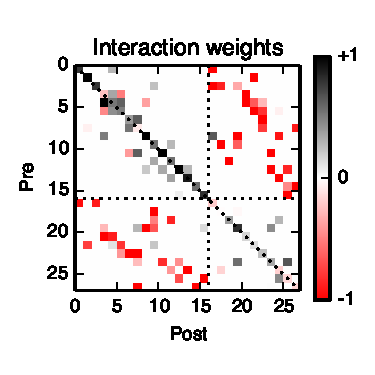
\includegraphics[width=\textwidth]{figure1a}
  \end{subfigure}
  ~
  \begin{subfigure}[T]{1.4in}
	    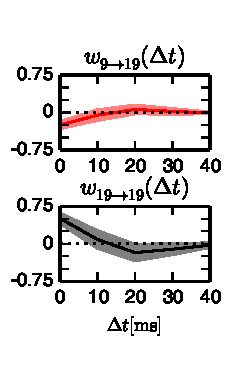
\includegraphics[width=\textwidth]{figure1c}
  \end{subfigure}
  ~
  \begin{subfigure}[T]{2.2in}
    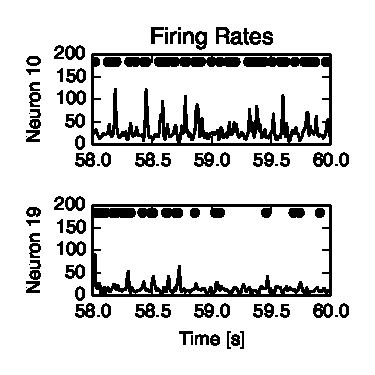
\includegraphics[width=\textwidth]{figure1b}
  \end{subfigure}
\vspace{-2.5em}
\caption{The negative binomial GLM applied to a population recording of retinal ganglion cells. Neurons~1--16 are ``OFF'' cells, and 17--27 are ``OFF'' cells.  The sparse network of inferred interactions is shown on the left, with canonical patterns of within-type excitation (black) and between-type inhibition (red). Each connection corresponds to a weighted impulse response, like those shown in the center. The sum of weighted impulse responses are passed through an exponential link function to determine the expected number of spikes per bin under the negative binomial model (right). }
\label{fig:figure1}
\vspace{-1.5em}
\end{figure}

\section{Bayesian Inference}
\citet{Pillow2012} have derived a data augmentation scheme to efficiently perform Bayesian inference in negative binomial regression models. The fundamental  property they exploit is that the likelihood as a function of~${\psi_{n,t}=\log \lambda_{n,t}}$ can be written as,
\begin{align}
p(s_{n,t} \given \psi_{n,t}, \xi) &\propto \frac{(e^{\psi_{n,t}})^{s_{n,t}}}{(1 + e^{\psi_{n,t}})^{s_{n,t} + \xi}}
 \propto  \exp \left(\frac{s_{n,t}-\xi}{2} \psi_{n,t}\right) \mathbb{E}_{\omega_{n,t}}\left[ \exp\left(-\omega_{n,t} \psi_{n,t}^2 / 2\right)\right],
\end{align}
where~${\omega_{n,t} \sim \text{PG} (s_{n,t}+\xi, 0)}$ and PG denotes the Polya-Gamma distribution. Hence, if we augment our data with Polya-Gamma random variables~${\omega_{n,t}}$, then conditioned on these variables the log likelihood is a quadratic function of~$\psi_{n,t}$ and conjugate with a Gaussian prior.  
~
% Commenting out the conditional distribution of \bpsi
\begin{comment}
Specifically, we have,
\begin{align}
\bpsi_n \given \bs_n, \boldsymbol{\omega}_n \sim \distNormal \left( \bbm_{\bpsi}, \bC_{\bpsi}  \right), 
\quad
\bbm_{\bpsi} = \bC_{\bpsi} \left[ \frac{\bs_n - \xi}{2}  + \frac{\bmu_{\bpsi}}{\sigma_{\bpsi}^2}\right], 
\quad
\bC_{\bpsi} = \left(\frac{1}{\sigma_{\bpsi}^2}\bI + \text{diag}(\boldsymbol{\omega}_n)\right)^{-1}.
\end{align}
\end{comment}
~
Similarly, the posterior distribution over~$\bomega_{n}$ factorizes into independent Polya-Gamma distributions that can be efficiently sampled.  This data augmentation scheme renders the our model conjugate and hence amenable to Gibbs sampling. The only exception is the spike-and-slab prior over~$A_{n'\to n}$ and~$\bw_{n'\to n}$. To improve the mixing of our Markov chain, we jointly update these parameters by marginalizing over the weights to sample~$A$ and then sampling~$\bw$ given~$A$. Since the weights and the likelihood are both Gaussian distributions, the marginal likelihood is also Gaussian and can be computed in closed form.  Integrating out weights removes the conditional independence of the elements of~$\bpsi_n$, but the resulting marginal distribution is Gaussian with a low rank plus diagonal covariance matrix, and hence can be efficiently inverted with the matrix inversion lemma.  

To demonstrate this approach, we have applied our negative binomial GLM to a population of primate retinal ganglion cells. With a simple Erd\H{o}s-Renyi network prior, we recover a sparse pattern of connectivity that filters out the insignificant interactions and leaves an obvious pattern of mutual excitation among cells of the same type (diagonal blocks) and inhibition between cells of different types (off-diagonal blocks), as shown in Figure~\ref{fig:figure1}. 

As we look toward increasingly large multiple spike train recordings, we plan to leverage many nice properties of this method. First, the data augmentation used to sample the negative binomial model is na\"ively parallelizable. Moreover, given the conjugacy of this model, stochastic variational inference is an appealing alternative to Gibbs sampling that combines the benefits of Bayesian inference with the scalability required to discover structure in large scale recordings. 

\vspace{-2em}
\renewcommand\refname{}
\bibliographystyle{imsart-nameyear}
{\small \bibliography{abstract}}

\end{document}

   
